\documentclass[12pt,a4paper,twoside]{book}
\usepackage{graphicx}
\usepackage{setspace}	%double spacing for text, single for captions, footnotes, etc.
%\usepackage{hypernat} 	%substitut de cite que permet fer hyperlinks
\usepackage{natbib}		% substituye a 'hypernat' que funciona en Windows.
\usepackage[spanish]{babel}
\usepackage[utf8]{inputenc}
\usepackage{color}
\usepackage{hhline} 		% extended styles for tables
\usepackage{multirow}
\usepackage{subfigure}
\usepackage{acronym}
\usepackage{hyperref}
\usepackage{amsmath,amsmath,amssymb} 
\usepackage{fancyhdr}
\usepackage{epsfig, amsmath}
\usepackage{algorithm}
\usepackage{algorithmic}

% general settings
\hypersetup{
	linktocpage=true,
	colorlinks=true,
	linkcolor=blue,
	citecolor=blue,
}
\definecolor{Hgray}{gray}{0.6}

\newenvironment{definition}[1][Definition]{\begin{trivlist}
\item[\hskip \labelsep {\bfseries #1}]}{\end{trivlist}}

\setlength{\topmargin}{0cm}
\setlength{\textheight}{23cm}
\setlength{\textwidth}{17cm}
\setlength{\oddsidemargin}{0cm}
\setlength{\evensidemargin}{0cm}
\setlength{\headheight}{1cm}

% Set numbered 'sub-sub-sections' and appear in the TOC
\setcounter{secnumdepth}{3}
\setcounter{tocdepth}{2}

% settings for code
\renewcommand{\algorithmicrequire}{\textbf{Input: }}
\renewcommand{\algorithmicensure}{\textbf{Output: }}

%%%%%%%%%%%%
% DOCUMENT %
%%%%%%%%%%%%
\begin{document}

% portada
\newpage
\thispagestyle{empty}

\baselineskip 2em

%\vspace*{1cm}

\centerline{
\includegraphics[width=0.6\textwidth]{ch0/UOC-logo}}
\begin{center}
\textsc{Universitat Oberta de Catalunya (UOC) \\
 Máster Universitario en Ciencia de Datos (\textit{Data Science})\\}

%\centerline {\pic{UOC}{4cm}}

\vspace*{1.5cm}

\textsc{\Large TRABAJO FINAL DE MÁSTER}

\vspace*{0.5cm}

\textsc{\large Área: Big Data / Machine Learning}


%\textbf{\Huge VirtualTechLab Model: }

\vspace*{2.0cm}

\textbf{\Large Automatic image descriptions}

\textbf{\large A deep-learning approach}

\vspace{2.5cm}
\baselineskip 1em

\baselineskip 2em
-----------------------------------------------------------------------------\\
Autor:      Mario Gómez Martínez\\
Tutor:      Anna Bosch Rué\\
Profesor:   Jordi Casas Roma\\
-----------------------------------------------------------------------------\\
\vspace*{1.5cm}
Valencia, \today

\end{center}

\newpage
\pagestyle{empty}
\hfill

\newpage
% abstract
\pagenumbering{roman} 
\setcounter{page}{1} 
\pagestyle{plain}

%%%%%%%%%%%%%%%%
%%% CREDITOS %%%
%%%%%%%%%%%%%%%%
\chapter*{Copyright}

\vspace{1cm}

\begin{figure}[ht]
    \centering
	
\includegraphics[scale=1]{ch0/license.png}
\end{figure}

This work is licensed under \href{https://creativecommons.org/licenses/by-nc-sa/3.0/es/deed.en}{Creative Commons Attribution-NonCommercial-ShareAlike 4.0 Spain License (CC BY-NC-SA 4.0 ES)} 

\vspace{1cm}

\begin{figure}[ht]
    \centering
	
\includegraphics[scale=1]{ch0/licencia.png}
\end{figure}

Esta obra está sujeta a una licencia de \href{https://creativecommons.org/licenses/by-nc-sa/4.0/es/}{Reconocimiento-NoComercial-CompartirIgual 4.0 España de Creative Commons (CC BY-NC-SA 4.0 ES)}


%%%%%%%%%%%%%
%%% FICHA %%%
%%%%%%%%%%%%%
\chapter*{FICHA DEL TRABAJO FINAL}

\begin{table}[ht]
	\centering{}
	\renewcommand{\arraystretch}{2}
	\begin{tabular}{r | l}
		\hline
		Título del trabajo: & Automated generation of image captions\\
		\hline
        Nombre del autor: & Mario Gómez Martínez\\
		\hline
        Nombre del colaborador/a docente: & Anna Bosch Rué\\
		\hline
        Nombre del PRA: & Jordi Casas Roma\\
		\hline
        Fecha de entrega (mm/aaaa): & 06/2019\\
		\hline
        Titulación o programa: & Máster en Ciencia de Datos\\
		\hline
        Área del Trabajo Final: & Aprendizaje automático\\
		\hline
        Idioma del trabajo: & Inglés\\
		\hline
        Palabras clave & Aprendizaje Profundo, Descripción de Imágenes\\
		\hline
	\end{tabular}
\end{table}

%%%%%%%%%%%%%%%%%%%
%%% DEDICATORIA %%%
%%%%%%%%%%%%%%%%%%%
\chapter*{Dedicatoria}

Dedicado a mi compañera, siempre ahí, para lo bueno y para lo malo, cercana, constante, inspiradora...

%%%%%%%%%%%%%%%%%%%
%%% Agradecimientos %%%
%%%%%%%%%%%%%%%%%%%
% \chapter*{Agradecimientos}

% Quisiera agradecer a...

%%%%%%%%%%%%%%%%
%%% RESUMEN  %%%
%%%%%%%%%%%%%%%%
\chapter*{Abstract}
\addcontentsline{toc}{chapter}{Abstract}

\onehalfspacing

Automatic image captioning, the task of automatically producing a natural-language description for an image, has the potential to assist those with visual impairments by explaining images using text-to-speech systems. However, accurate image captioning is a challenging task that requires integrating and pushing further the latest improvements at the intersection of computer vision and natural language processing fields

This work aims at building an advanced model based on neural networks and deep learning for the automated generation of image captions. 


\vspace{1.5cm}

\textbf{Keywords}: Deep Learning, Artificial Neural Networks, Automated image captioning


\chapter*{Resumen}
\addcontentsline{toc}{chapter}{Resumen}

\onehalfspacing

El subtitulado automático de imágenes, la tarea de producir automáticamente una descripción en lenguaje natural para una imagen, tiene el potencial de ayudar a las personas con discapacidades visuales a explicar las imágenes mediante sistemas de conversión de texto a voz. Sin embargo, el subtitulado preciso de imágenes es una tarea desafiante que requiere integrar y avanzar en la intersección de los campos de procesamiento de lenguaje natural y visión por computador.

Este trabajo pretende desarrollar un modelo basado en redes neuronales y aprendizaje profundo para la generación automática de descripciones de imágenes.


\vspace{1.5cm}

\textbf{Palabras clave}: Aprendizaje Profundo, Redes Neuronales Artificiales, Descripción automática de imágenes
\newpage

\pagestyle{fancy}
\renewcommand{\chaptermark}[1]{ \markboth{#1}{}}
\renewcommand{\sectionmark}[1]{\markright{ \thesection.\ #1}}
\lhead[\fancyplain{}{\bfseries\thepage}]{\fancyplain{}{\bfseries\rightmark}}
\rhead[\fancyplain{}{\bfseries\leftmark}]{\fancyplain{}{\bfseries\thepage}}
\cfoot{}

% indice
\cleardoublepage
\phantomsection
\addcontentsline{toc}{chapter}{Index}
\tableofcontents
% listado de figuras
\cleardoublepage
\phantomsection
\addcontentsline{toc}{chapter}{List of Figures}
\listoffigures
% listado de tablas
\cleardoublepage
\phantomsection
\addcontentsline{toc}{chapter}{List of Tables}
\listoftables

\thispagestyle{empty}

\pagenumbering{arabic}

\pagestyle{fancy}
\renewcommand{\chaptermark}[1]{ \markboth{#1}{}}
\renewcommand{\sectionmark}[1]{\markright{ \thesection.\ #1}}
\lhead[\fancyplain{}{\bfseries\thepage}]{\fancyplain{}{\bfseries\rightmark}}
\rhead[\fancyplain{}{\bfseries\leftmark}]{\fancyplain{}{\bfseries\thepage}}
\cfoot{}

\onehalfspacing

% capitulos del documento
\chapter{Introduction}
\label{chapter:introduccion}

\section{Motivation}

The web provides a vast amount of information, including a lot of text, but it is increasingly dominated by visual information, both static (pictures) and dynamic (videos).  However, much of that visual information is not accessible to those with visual impairments, or with slow internet speeds that prohibit the loading of images. Image captions, manually added by content providers (typically by using the \textit{ Alt-text} HTML tag), is one way to make this content more accessible, so that a natural-language description of images and videos can be presented using \textit{text-to-speech} systems. However, existing human-curated image descriptions are added for only a very small fraction of web images. Thus, there is great interest in developing methods to automatically generate image descriptions.

Automatic image description can be defined as the task of automatically generating a description of an image using natural language. It is a very challenging problem that encompasses two kind of problems: the problem of understanding an image, which is a Computer Vision (CV) task, and the problem of generating a meaningful and grammatically-correct description of the image, which is a kind of Natural-Language Processing (NLP) task . Therefore, to tackle this task it is necessary to advance the research in the two fields, CV and NLP, as well as promoting the cooperation of both communities to address the specific problems arising when combining both tasks.

Figure \ref{fig:image-captioning} shows an example of the automatic image generation tasks addressed by this project.

\begin{figure}
	\centering
	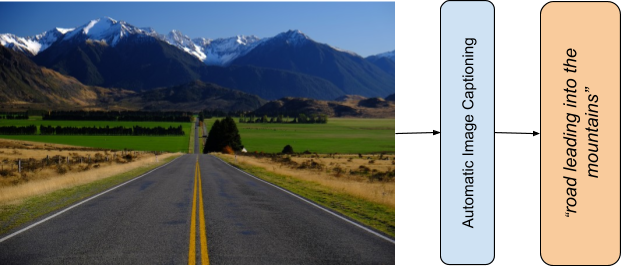
\includegraphics[width=0.6\textwidth]{figs/ch1/image-captioning.png}
	\caption{Image captioning can help millions with visual impairments by converting images captions to text. Image by \href{https://www.flickr.com/photos/francisvallance/}{Francis Vallance (Heritage Warrior)}, used under \href{https://creativecommons.org/licenses/by/2.0/}{CC BY 2.0 license}.}
	\label{fig:image-captioning}
\end{figure}

In addition to the aforementioned application of image captioning to help the visually impaired, there are many other use cases in which automatic image descriptions may help. In general, any domain in which images need to be interpreted by humans, but human availability is scarce or it is a tedious task, may benefit from an automated approach to image description.

A specific use case is the analysis and extraction of information from videos. Some video monitoring tasks are very boring and tedious. An automated mechanism to describe scenes in video footage will be of great utility for creating summaries or monitoring specific situations and events. \footnote{As an interesting example, Shell is conducting a pilot study using deep-learning to automatically monitor video footage in order to identify safety hazards and generate alerts (\href{https://customers.microsoft.com/en-us/story/shell-mining-oil-gas-azure-databricks}{link})}.

Another potential utility of automatic image description lies in the task of searching images. Having automatically generated captions for images that originally hasn't been described, would help finding images based on a complex description rather that a simple collection of tags.

\section{Goals}

This project aims at advancing in the task of automatically generating image descriptions. That is the ultimate goal of the project. However, in order to achieve such an abstract goal, we decompose it into various subgoals, as follows:

\begin{enumerate}
\item Get a solid understanding of the problem at hand and review the state-of-art solutions to it
\item Get practical knowledge on the technologies required to solve this problem
\item Develop a model using a benchmark dataset like the Flickr30K
\item Scale the model to a larger benchmark dataset such as the COCO\cite{Lin2014} dataset or the more recent Conceptual Captions Dataset by Google \cite{Sharma2018}  (see Figure \ref{fig:conceptual-captions}).
\item Evaluate the model, ideally partaking in some challenge or competition, like the ones using the COCO dataset or the Conceptual Captions dataset.
\end{enumerate}

\begin{figure}[h]
	\centering
	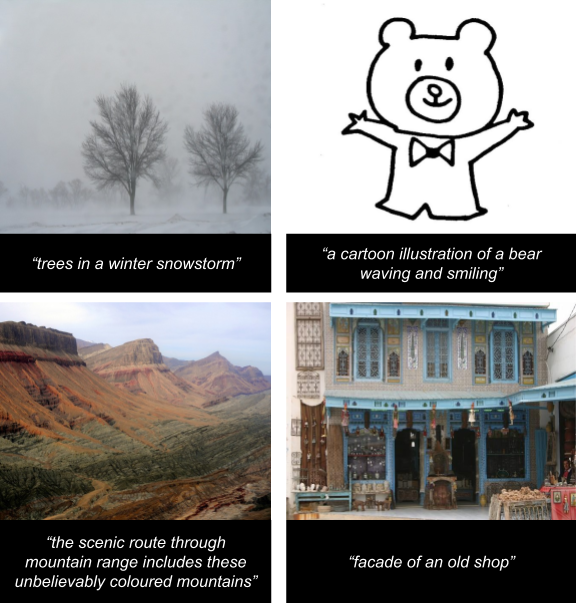
\includegraphics[width=0.6\textwidth]{figs/ch1/conceptual-captions-example.png}
	\caption{Illustration of images and captions in the Conceptual Captions dataset.Clockwise from top left, images by Jonny Hunter, SigNote Cloud, Tony Hisgett, ResoluteSupportMedia. All images used under \href{https://creativecommons.org/licenses/by/2.0/}{CC BY 2.0 license}.}
	\label{fig:conceptual-captions}
\end{figure}

\section{Methodology}

This project is mainly an academical, research-oriented project, so it would follow a process model which is common for these kind of projects, for instance, it will include a comparatively long review of the state of the art, as well as a public defense at the end. However, this project will also include the development of a software artifact to solve a data-analytic problem, therefore we should benefit from using a data-analytic model as the well known and widely adopted \textbf{CRISP-DM}. CRISP-DM, which stands for \textit{Cross-Industry Standard Process for Data Mining}, is an open standard process model and an industry-proven methodology to guide data mining projects.

As a methodology, it includes descriptions of the typical phases of a project, the tasks involved with each phase, and an explanation of the relationships between these tasks.

As a process model, CRISP-DM provides an overview of the data mining life cycle.

Figure \ref{fig:crisp-dm} depicts the relationships between the different phases of the CRISP-DM model. The sequence of the phases is not strict and moving back and forth between different phases is often required. The arrows in the process diagram indicate the most important and frequent dependencies between phases. The outer circle in the diagram symbolizes the cyclic nature of data mining itself. A data mining process continues after a solution has been deployed. The lessons learned during the process can trigger new, often more focused business questions, and subsequent data mining processes will benefit from the experiences of previous ones.

\begin{figure}[hpt]
	\centering
	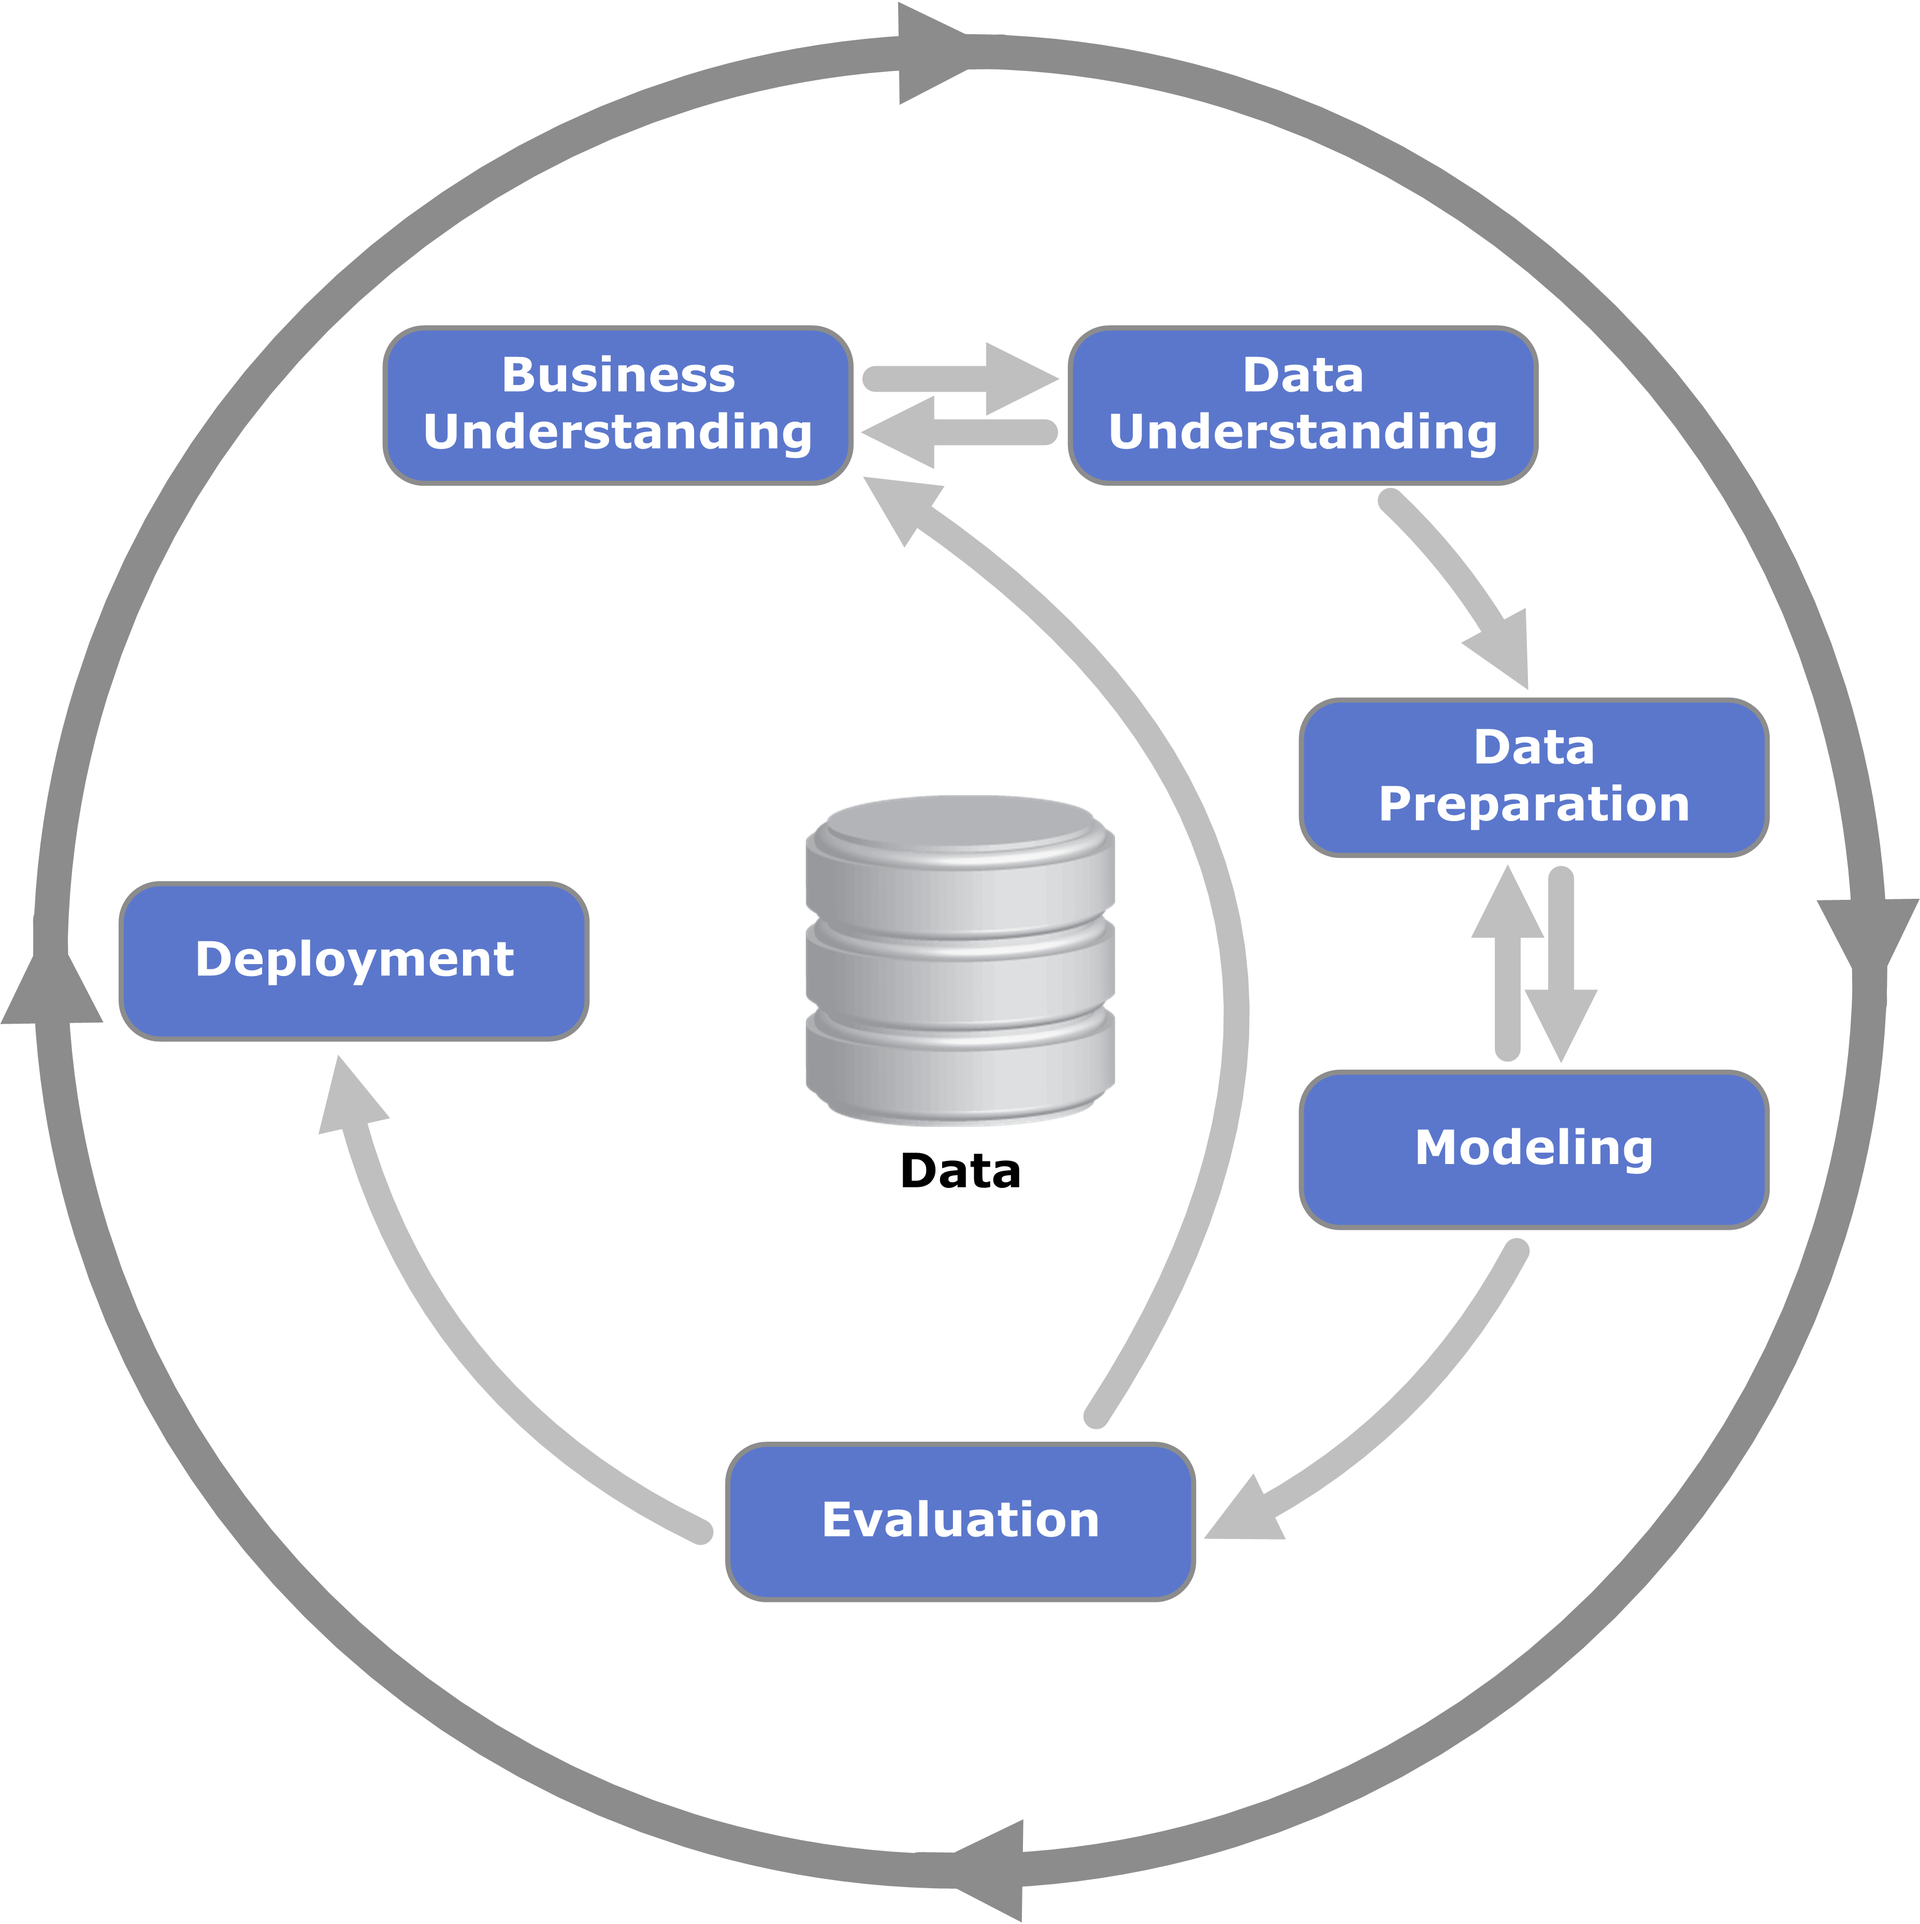
\includegraphics[width=0.6\textwidth]{figs/ch1/crisp-dm.png}
	\caption{Process diagram showing the relationship between the different phases of CRISP-DM. Image by Kenneth Jensen, used under \href{https://creativecommons.org/licenses/by/2.0/}{CC BY-SA 3.0 license..}}
	\label{fig:crisp-dm}
\end{figure}

The process model consists of six major phases:

\begin{itemize}
\item \textbf{Business Understanding}: Includes an in-depth analysis of the business objectives and needs. The situation is assessed and the goals of the project are defined. This should follow the setting up of a plan to proceed.
\item \textbf{Data Understanding}: Conduct initial or exploratory data analysis to become familiar with data and identify potential problems. Examine properties of data and verify its quality by answering questions concerning the completeness and accuracy of the data.
\item \textbf{Data Preparation}: After the data sources are completely identified, proper selection, cleansing, constructing and formatting should be done before modelling. 
\item \textbf{Modeling}: Modeling is usually conducted in multiple iterations, which involve running  several models using the default parameters and then fine-tune the parameters or revert to the data preparation phase for additional preparation. Usually, there are different ways to look at a given problem, so it is convenient to build multiple models,
\item \textbf{Evaluation}: The results of models are evaluated in the backdrop of business intentions. New objectives may sprout up owing to the new patterns discovered. This is, in fact, an iterative process, and the decision whether to consider them or not has to be made in this step before moving on to the final phase
\item \textbf{Publication}. The final information gathered has to be presented in a usable manner to the stakeholders.  This has to be done as per their expectations and business requirements.
\end{itemize}


\section{Planning}

Main tasks and milestones

\begin{table}[hbt]
\begin{tabular}{|l|l|l|}
\hline
Phase   & End  & Description   \\ \hline
1 & 3/3/2019 & Definition and planning  \\ \hline
2 & 24/3/2019 & State of the Art \\ \hline
3 & 19/5/2019 & Development \\ \hline
4 & 9/6/2019 & Complete this report \\ \hline
5 & 16/6/2019 & Presentation
\end{tabular}
\end{table}

Phase 2: this phase will encompass the following tasks:
\begin{itemize}
\item Reviewing relevant bibliography
\item Studying the problem domain (business understanding), and becoming familiar with the data. At this stage we would also start preparing the data for the modeling stage
\end{itemize}

Phase 3: this will be the longest phase, and it will include the following tasks  
\begin{itemize}
\item Preparing the data. Although data preparation could be started during phase 2, depending on the chosen models it could be necessary to conduct some additional data preparation operations
\item Generating one or various models. We plan at creating at least two models, one that would replicate existing work, and another one to explore new ideas and try to beat the baseline model.
\item Evaluating the models, and very specifically, compare our model against the replicated model.
\item Publication: We consider two courses of action: a) participating in the Conceptual Captions Challenge by Google, and b) delivering some product to the final user, although it would be a very basic prototype given the little time available.
\end{itemize}

In phase 4 we will complete this report. We would probably overlap this task with some of the tasks in phase 3 that will required more time, like the evaluation of the models and the participation in challenges.

In phase 5 we will present the results achieved for its evaluation. These results will include the code, the documentation and a public defense of the project in front of an academic board



% bibliografia
\addcontentsline{toc}{chapter}{Bibliography}
\bibliographystyle{plain}
\bibliography{references}

\end{document}